\documentclass[cjk,c,squeeze,shrink,dvipdfmx,12pt]{beamer}
% 以下は決まり文句
\usepackage{bxdpx-beamer}                      % dvipdfmx用の fix
\usepackage{pxjahyper}                         % 日本語で'しおり'
\usepackage{minijs}                            % min10ヤダ
\renewcommand{\kanjifamilydefault}{\gtdefault} % 既定をゴシック体に

\usetheme{KansaiDebian}
\usepackage{amsmath,amssymb,ulem}
\AtBeginSection[]{%
  \begin{frame}<beamer>\frametitle{Outline}\tableofcontents[currentsection]\end{frame}}

\title{Debian Updates}
\subtitle[]{〜第116回オープンソースサロン〜}
\author[佐々木]{%
  佐々木洋平/Youhei SASAKI\newline
  twitter/github: \alert{@uwabami}
}
\institute[Debian JP Project]{%
  Debian JP Project/関西Debian勉強会\\
  {\color{blue}{uwabami@debian.or.jp}}
}
\date[2017/12/08]{%
  {\footnotesize{2017年12月8日@イチバタダイニング}}
}

\begin{document}
\setbeamercovered{transparent}
\takahashi[80]{ }
{%
  \setbeamertemplate{headline}{}
  \setbeamertemplate{footline}{}
  \begin{frame}
    \maketitle
  \end{frame}
}

\begin{frame}[fragile]{Outline}
  \tableofcontents
\end{frame}
%-------------------

\section{Debianとは?}
\takahashi[60]{Debianとは?}

\begin{frame}[fragile]{Debian とは?}

  \alert{フリー/オープン}な\alert{ユニバーサル}オペレーティングシステムを
  作成しようとするボランティアベースのプロジェクト。

  \vfill
  \centering
  \begin{tabular}{|c|c|c|}
    \hline
    ディストリ & 企業 & ボランティア \\ \hline
    RHEL & RedHat & なし  \\ \hline
    CentOS & RedHat & あり \\ \hline
    Ubuntu  & Canonical & あり \\ \hline
    \alert{Debian}  & \alert{なし} & \alert{あり} \\ \hline
  \end{tabular}
  \vfill
\end{frame}


\begin{frame}[fragile]{Debian とは?}
Linux カーネルだけではなく、FreeBSD や GNU/Hurd のカーネルを利用したOSも提供。

\centering
% ビルド前に画像を get しておくこと.
% \includegraphics[width=.2\paperwidth]{image201711/625px-NewTux.png}
% \includegraphics[width=.5\paperwidth]{image201711/523px-Freebsd_logo.png}
% \includegraphics[width=.2\paperwidth]{image201711/Hurd-logo.png}
\end{frame}


\begin{frame}[fragile]{Debian とは?}

  厳格/厳密なポリシーとガイドラインに沿った開発体制
  \begin{itemize}
  \item Debian 社会契約
  \item Debian フリーソフトウェアガイドライン
    \begin{itemize}
    \item オープンソースの定義の元
    \end{itemize}
  \item Debian Policy
  \end{itemize}

\end{frame}

\begin{frame}[fragile]{Debian とは?}
  \begin{columns}
    \begin{column}{.58\paperwidth}
      \begin{itemize}
      \item
        Ubuntu や Raspbian といったディストリビューションのベースとなっている
      \item
        Debian Derivatives(Debian 派生ディストリビューション)との協力体制の整備
      \end{itemize}
    \end{column}
    \begin{column}{.4\paperwidth}
      \centering
      % \includegraphics[height=.65\paperheight]{image201711/500px-DebianFamilyTree1210.png}
    \end{column}
  \end{columns}
\end{frame}


\begin{frame}[fragile]{Debian とは?}
 世界規模で開発が行われており、63ヶ国、約1000名のDebian公式開発者が開発を行
 っている。パッケージメンテナや翻訳などの貢献者も入れるともっと多くの開発者が参加
 していることになる。

 \centering
 % \includegraphics[width=0.8\linewidth]{image201711/debconf_2017.jpg}
\end{frame}


\begin{frame}[fragile]{Debian とは?}
  2017年11月の時点で、
  \pause
  \begin{itemize}[<+->]
  \item
    最新版は {\alert{Debian 9.2}}, Stretch
  \item
    提供パッケージ数は{\alert{約51000}}
  \item
    公式にサポートするCPUアーキテクチャは{\alert{10}}
  \item {\alert{約2年毎}}にリリース
  \item next: Debian 10, Buster は2019年にリリース予定
  \item コードネームはトイ・ストーリーのキャラクターから
  \end{itemize}
\end{frame}

\begin{frame}[fragile]{Debianとは?}
\centering
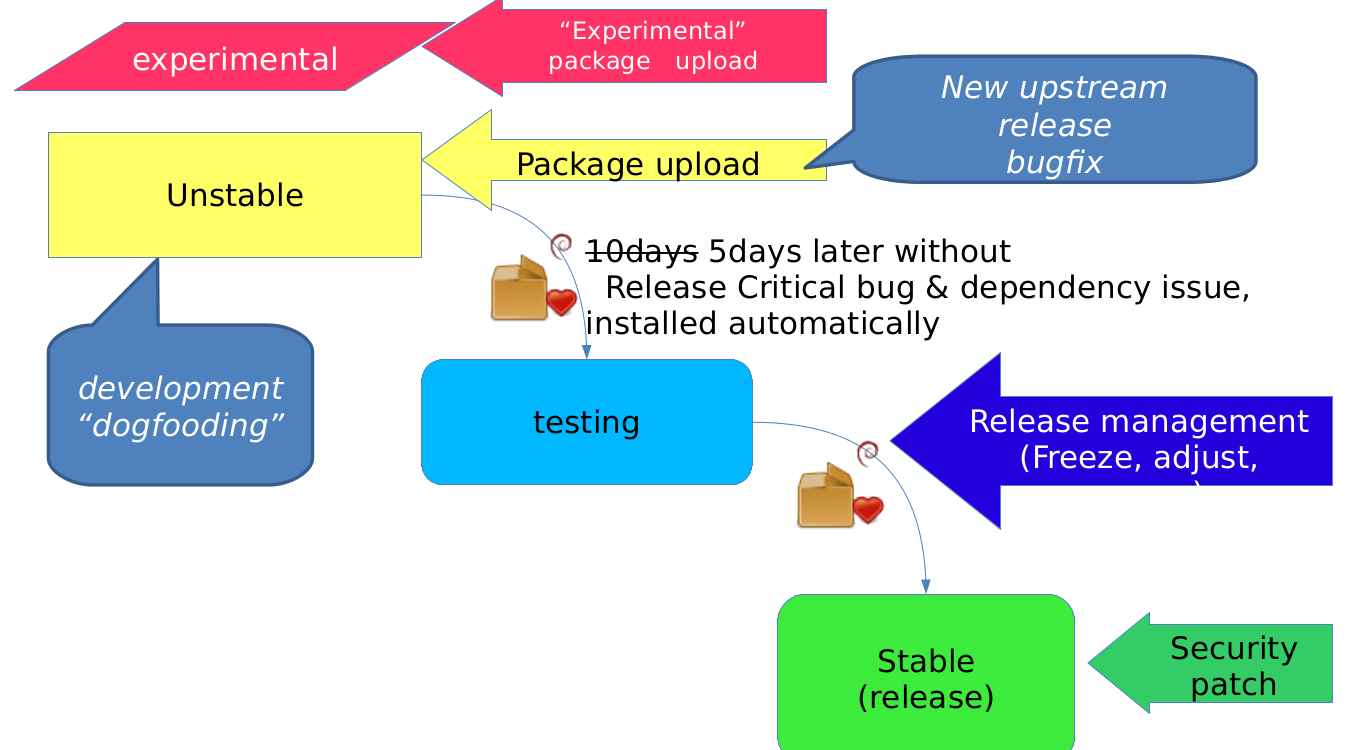
\includegraphics[width=.98\textwidth]{image201712/release-cycle.png}
\end{frame}

\begin{frame}[fragile]{Debian とは?: まとめ}
  \pause
  \begin{itemize}[<+->]
  \item Debianはフリー/オープンなOSを作成しようとするボランティアベースのプロジェクト。
  \item 自分たちの考えるフリーという言葉に関する定義、開発目的、パッケージングポリシーを厳格に決めている。
  \item 世界中に1000人以上の開発者がおり、他のディストリビューションのベースとして採用されている。
  \item 約2年毎にリリースが行われ、多くのパッケージとアーキテクチャをサポートしている。  \item 上記のような特徴から様々なところで利用されているLinuxディストリビューションである。
\end{itemize}
\end{frame}

\iffalse
%------------------
\begin{frame}[fragile]{Debian JP Project とは?}
  \pause
  \begin{itemize}[<+->]
  \item 日本でのDebianの普及を目的とした任意団体。
  \item %
    Debianの日本語による情報発信、
    ユーザとの情報交換、
    Debian 開発者、
    パッケージメンテナの育成など。
  \end{itemize}
\end{frame}


\begin{frame}
  \frametitle{Debian勉強会}
  \begin{itemize}
  \item 2005年1月開始
  \item Debian Developer 上川さん発起人
  \item 東京と関西で月に一回コンスタントに開催しているDebian開発者、ユーザによる勉強会。
  \end{itemize}
\end{frame}

\begin{frame}

  \frametitle{Debian勉強会:解決したい内容}
  \begin{itemize}[<+->]
  \item 問題
    \begin{itemize}
    \item MLとIRCで情報交換していた
    \item face-to-faceであう場所がない
    \item まとまったドキュメントが出てこない
    \end{itemize}
  \item Debian勉強会の提案
    \begin{itemize}
    \item 定期的に集まる
    \item 資料を作成する。(GPLで!) \\
      {\small \url{git://anonscm.debian.org/tokyodebian/monthly-report.git}}
    \end{itemize}
  \end{itemize}

\end{frame}
\fi
% \begin{frame}
%  \frametitle{Debian勉強会:実際}
%  \begin{itemize}
%   \item Debian Weekly News Quiz
%   \item Debian 界隈やパッケージング関連の話題など専門の人に話を聞く
%   \item 前回の内容(東京 8月):\\
%     \begin{itemize}
%     \item 場所: 朝日ネットさん
%     \item 「debconf17参加報告」(青木さん、やまねさん)
%     \end{itemize}
%   \item 各地のイベントでDebian普及活動
%     \begin{itemize}
%       \item OSC2016群馬、OSC2016沖縄、OSC2017北海道など
%       \item Debian/Ubuntu ユーザミートアップ in 札幌を開催
%     \end{itemize}
%  \end{itemize}
% \end{frame}

%-----------------------
\takahashi[40]{Any Questions?}
\section{Debian 9 (Stretch)}

\takahashi[40]{Debian 9 (Stretch)}

\begin{frame}[fragile]{Debian 9 について: R.I.P. Ian Murdock}
  \begin{itemize}
  \item %
    Debian 9.0 (コードネーム:Stretch) は 2017-06-17にリリース
  \item %
    このリリースは、Debian Projectの創始者 Ian Murdock氏に捧げるリリースになっている。
  \end{itemize}
  \begin{quote}
    $\cdots$\\
    Ian Murdock, the founder of the Debian project, passed away on 28th
    December 2015 at his home in San Francisco. He was 42.
    $\cdots$\\
    \flushright{\texttt{https://www.debian.org/News/2017/20170617}}
  \end{quote}
\end{frame}


\begin{frame}[fragile]{Debian 9 について: Arch. support status}% [containsverbatim]

\begin{itemize}
\item i386アーキテクチャのサポートCPUをi686以降に変更
\item サポートされるアーキテクチャ
  \begin{itemize}
  \item
    amd64, i386, armel, armhf, arm64, mips,
    mipsel, {\alert{mips64el}}, ppc64el, s390x
  \end{itemize}
\item サポートから外れたアーキテクチャ
  \begin{itemize}
  \item
    powerpc
  \end{itemize}
\end{itemize}
\end{frame}


\begin{frame}[fragile]{Debian 9 について: Arch. support status}% [containsverbatim]

  \centering
  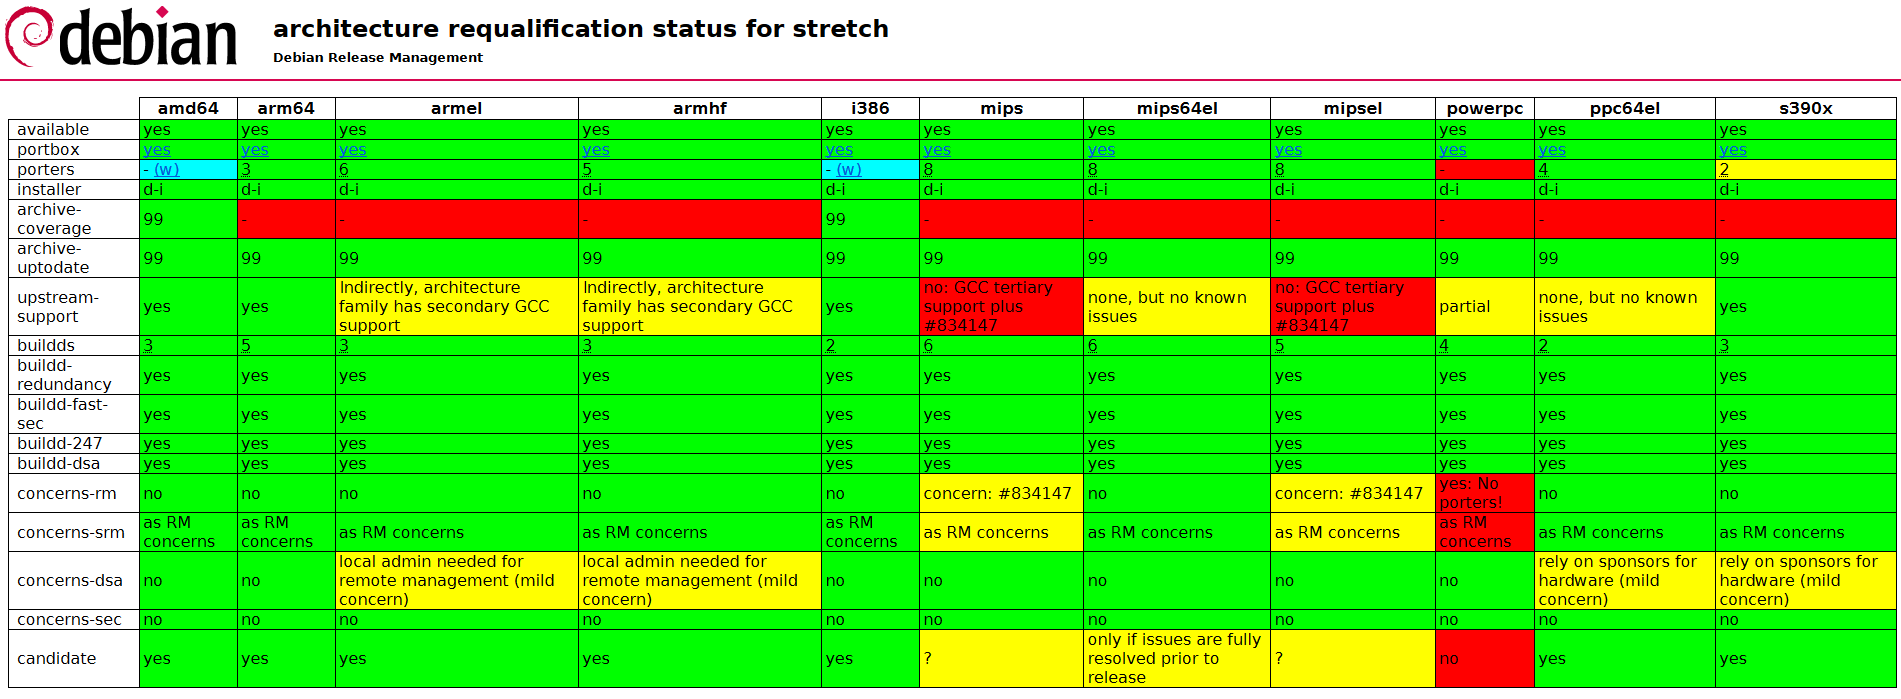
\includegraphics[width=1.0\hsize]{image201707/stretch-arch-requalification.png}
\end{frame}

\begin{frame}[fragile]{Debian 9 について: Theme}% [containsverbatim]
  \centering
  % \includegraphics[width=0.75\hsize]{image201711/attachment_wallpaper.png}
  % \newline
  {\small{``Soft waves'' by Juliette Taka Belin}}
\end{frame}


\begin{frame}[fragile]{Debian 9 について: 主なソフトウェア}% [containsverbatim]

\begin{itemize}
\item Linux カーネルは 4.9
\item ツールチェイン(GCC 6.3.0, binutils 2.28, glibc 2.24), LLVM 3.7.1, 3.8.1, 3.9.1
\item Perl 5.24.1, Python 2.7.13/3.5.3, Ruby 2.3.3, PHP 7.0.19, Go 1.7.4, OpenJDK 8
\item GNOME 3.22, KDE 5.8, Xfce 4.12.3, lxde 0.99.0, lxqt 0.11.1
\item MariaDB 10.1.23, PostgreSQL 9.6.3, sqlite 3.15
\item OpenSSL 1.1.0, GnuPG 2.1.18/1.4.21
\item クロスコンパイラがデフォルトでサポート
\item etc..
\end{itemize}

\end{frame}


\begin{frame}[fragile]{Debian 9 について: 主な変更点}% [containsverbatim]

\begin{itemize}
\item iproute2が推奨\\
 ← net-toolsは非推奨(例:ifconfig、arp、netstat、route)
\item iceweasel → firefox、icedove → thunderbirdという名称で提供
\item mysqlパッケージは提供されず、mariadbパッケージのみを提供
  \begin{itemize}
  \item jessieからアップグレードする場合は、自動でmariadbパッケージに置き換えられる
  \item データベースは自動変換されるが、元に戻せないこと、失敗することもありうることを想定し、データ保全は各自の責任で実施すること
  \end{itemize}
\item Xorg サーバはroot権限でなくユーザ権限で動作することが可能
\end{itemize}
\end{frame}


\begin{frame}[fragile]{Debian 9 について: セキュリティ関係}% [containsverbatim]

\begin{itemize}
\item ウェブブラウザはセキュリティ更新が提供されるFirefoxおよびChromiumの利用を推奨
\item Firefox及びThunderbirdは、ESR版のセキュリティ更新を提供
\item libv8-3.14、nodejs、node-*はセキュリティ更新が提供されない
\item OpenSSLにおいて 3DES、RC4 暗号は TLS/SSL 通信には利用できない
\end{itemize}

\end{frame}


\begin{frame}[fragile]{Debian 9 について: 互換性}% [containsverbatim]

\begin{itemize}
\item ネットワークインタフェース名がenp1s1、wlp3s0 のように変更
  \begin{itemize}
  \item ただし、Debian 8 Jessieからアップグレードした場合は、eth0、wlan0といった昔の命名規則で据え置き
  \end{itemize}
\item OpenSSHは標準で旧式の暗号とSSH1プロトコルが無効
  \begin{itemize}
  \item 古いsshクライアントから接続できなくなる可能性がある. 要確認
  \end{itemize}
\item X Window Systemのinputドライバがlibinputに変更
  \begin{itemize}
  \item Debian 8 jessieではevdevを採用
  \end{itemize}
\item Upstartは削除
  \begin{itemize}
  \item systemd(デフォルト)、SysVinit、OpenRCが利用可能
  \end{itemize}
\end{itemize}

\end{frame}


\begin{frame}[fragile]{Debian 9 について: 開発関連}% [containsverbatim]
  \begin{itemize}
  \item debhelper 10
    \begin{itemize}
    \item パラレルビルドがデフォルト化
    \item autoreconfをデフォルトで実行するように変更
    \item パッケージビルド時はdbgsymパッケージの生成をデフォルト化
    \item 生成したdbgsymパッケージは以下のapt-lineを指定して取得\\
      {\footnotesize{%
          \texttt{deb http://debug.mirrors.debian.org/debian-debug/ stretch-debug main}}}
    \item  dh\_installinit コマンドの
      \texttt{--restart-after-upgrade} オプションがデフォルト化
    \end{itemize}
  \item 実行ファイルはデフォルトで PIE を有効にしてコンパイル及びリンクしている
  \end{itemize}
\end{frame}


\begin{frame}[fragile]{Debian 9 について: インストーラ}% [containsverbatim]

\begin{itemize}
\item GUIインストールがデフォルト
\item UEFIのセキュアブートは未対応
\item screen対応
\item multiarchのインストーラは、amd64をデフォルトでインストール
\item HTTPSミラーからパッケージのダウンロードが可能
\item 全バイナリパッケージを提供するISOファイルからCD用のイメージを廃止
  \begin{itemize}
  \item DVDイメージ、blu-rayイメージのみの配布
  \item CDイメージは、
    netinst及びxfce4のみのデスクトップ環境を収録したCD一枚に収まる形でのみ提供
  \end{itemize}
\end{itemize}

\end{frame}


\begin{frame}[fragile]{Debian 9 について: アップグレード}% [containsverbatim]

  \begin{itemize}
  \item \alert{リリースノートを読む}
  \item apt-lineが \texttt{ftp://} の場合は、\texttt{http://} へ変更
  \item 利用環境がjessieより前の場合には, 先ずJessieにアップグレード
    \begin{itemize}
    \item メジャーバージョンの飛ばしアップグレードは非対応
    \end{itemize}
  \item debian $>=$ 8.8以降にアップグレードし, 必ずreboot\\
     ← PIE 対応のため
  \item debian 9へのアップグレードはupgrade、dist-upgradeの2段階
  \end{itemize}
\end{frame}


\begin{frame}[fragile]{Debian 9 について}% [containsverbatim]
  \Large
  \begin{center}
    何かおかしい動作や不具合を見つけた場合は\\
    Bug Reportをお願いします
  \end{center}
\end{frame}

\takahashi[40]{Any Questions?}
%-----------------------

\section{Debian Updates}
\takahashi[60]{Debian Updates}


\begin{frame}[fragile]{Debian Updates: Jessie}% [containsverbatim]
\pause
\begin{itemize}[<+->]
\item 2017/01/14: Updated Debian 8.7 released
\item 2017/05/06: Updated Debian 8.8 released
\item 2017/07/22: Updated Debian 8.9 released
\item[] :
\item \alert{2018/06/17: EOL}
\item[←] oldstable のサポートは stable リリース後 1 年
\item[※] その後は LTS へ以降(予定)
\end{itemize}

\end{frame}


\begin{frame}[fragile]{Debian Updates: DPL elections}% [containsverbatim]
  \begin{itemize}[<+->]
  \item 2017/4/15:  Debian Project Leader Elections 2017 投票
    \begin{itemize}
    \item %
      2017年のDebianプロジェクトリーダー(DPL)を決める選挙が行われ、Chris Lambさんが選出されました。
      選挙における声明は、\url{https://www.debian.org/vote/2017/platforms/lamby} を参照。
    \end{itemize}
  \end{itemize}
\end{frame}


\begin{frame}[fragile]{Debian Updates: shutdown FTP}% [containsverbatim]
  \begin{itemize}[<+->]
  \item 2017/04/25:  Shutting down public FTP services
    \begin{itemize}
    \item %
      ftp://ftp.debian.org、
      ftp://security.debian.orgのFTPサービスは 2017/11/01に停止
    \item %
      HTTPサービスは継続するため、
      ftpを使っているユーザはapt-lineを"http://"に変更しよう
    \end{itemize}
  \end{itemize}
\end{frame}

\begin{frame}[fragile]{Debian Updates: Stretch}% [containsverbatim]
  \begin{itemize}[<+->]
  \item 2017/06/17:  Debian 9 「Stretch」 released
  \item 2017/06/18:  Debian GNU/Hurd 2017 released
    \begin{itemize}
    \item
      Debian 9 Stretchがリリースされた翌日に、
      sid(=unstable)のsnapshotとしてDebian GNU/Hurd 2017がリリース
    \end{itemize}
    % https://lists.debian.org/debian-hurd/2017/06/msg00017.html
  \item 2017/07/22:  Debian 9.1 released
    % https://lists.debian.org/debian-release/2017/07/msg00294.html
  \item 2017/10/07:  Debian 9.2 released
  \end{itemize}
\end{frame}

\begin{frame}[fragile]{Debian Updates: Debconf}% [containsverbatim]
  \begin{itemize}[<+->]
  \item 2017/8/6-8/12:  debconf17
    \begin{itemize}
    \item
      debconf17をカナダ モントリオールで開催。
      webサイトでビデオを公開中。\url{https://debconf17.debconf.org/}
      % \newline
      % \includegraphics[width=0.6\linewidth]{image201711/debconf_2017.jpg}
    \end{itemize}
  \item
    ※\uline{debconf18: 台湾 新竹市(Hsinchu), 2018/07/29 - 08/04}
  \end{itemize}
\end{frame}

\takahashi[40]{Any Questions?}
\section{日本語によるDebianの情報}
\takahashi[40]{日本語によるDebianの情報}

\begin{frame}[fragile]{日本語によるDebianの情報}
  \begin{itemize}
  \item Debian JP Project \\
    \url{http://www.debian.or.jp}
  \item 東京エリアDebian勉強会\\
    \url{http://tokyodebian.alioth.debian.org}
  \item 関西エリアDebian勉強会 \\
    \url{https://wiki.debian.org/KansaiDebianMeeting}
  \item Twitter \\
    \url{@debian_jp}
  \item G+ コミュニティ \\
    \url{https://plus.google.com/u/0/communities/106942835439686570073}
  \end{itemize}
\end{frame}

\begin{frame}
  \frametitle{書籍情報}
  \begin{columns}
    \begin{column}{.5\paperwidth}
      \centering
      % \includegraphics[height=.6\paperheight]{image201711/SD201711.jpg}
    \end{column}
    \begin{column}{.5\paperwidth}
      \begin{itemize}
      \item %
        日本語での唯一の連載記事 \\
        「Debian Hot Topics」
      \end{itemize}
    \end{column}
  \end{columns}
\end{frame}

\begin{frame}
  \frametitle{書籍情報}
  \begin{columns}
    \begin{column}{.45\paperwidth}
      \centering
      % \includegraphics[height=.6\paperheight]{image201711/DebianHandbook.jpg}
    \end{column}
    \begin{column}{.54\paperwidth}
      \begin{itemize}
      \item %
        英語書籍の翻訳版
        \begin{itemize}
        \item %
          原版: The Debian Administrator's Handbook
          \begin{itemize}
          \item %
            Rapha\"el Hertzog, Roland Mas
          \item \url{https://debian-handbook.info/}
          \end{itemize}
        \end{itemize}
      \item %
        日本語で読める(現状)唯一の書籍!
      \item %
        パッケージ版:
        \texttt{debian-handbook}
      \end{itemize}
    \end{column}
  \end{columns}
\end{frame}


%----------------
\iffalse
\section{今後のイベント}

\takahashi[50]{今後のイベント}

\begin{frame}[fragile]{今後のイベント}
  \begin{block}<2->{11/18 第157回東京エリアDebian勉強会@横浜}
    \begin{itemize}
    \item \alert{DPLのChris Lambさんがゲストとして参加されます!!}
    \item \url{https://debianjp.connpass.com/event/70414/}
    \item ※前日には来日記念宴会もあります
      % \begin{itemize}
      % \item Debianプロジェクトリーダー来日記念宴会11/17@横浜
      % \item \url{https://debianjp.connpass.com/event/70413/}
      % \end{itemize}
    \end{itemize}
  \end{block}
  \vfill
  \begin{block}<3->{11/26 第129回関西Debian勉強会@大阪}
    \begin{itemize}
    \item 福島区民センター 304号室
    \item \url{https://debianjp.connpass.com/event/71914/}
    \end{itemize}
  \end{block}
  \vfill
\end{frame}
\fi
\takahashi[40]{Any Questions?}
\takahashi[60]{Thanks!!}

\takahashi[80]{ }

\end{document}
